\begin{figure}[tbp]
\centering
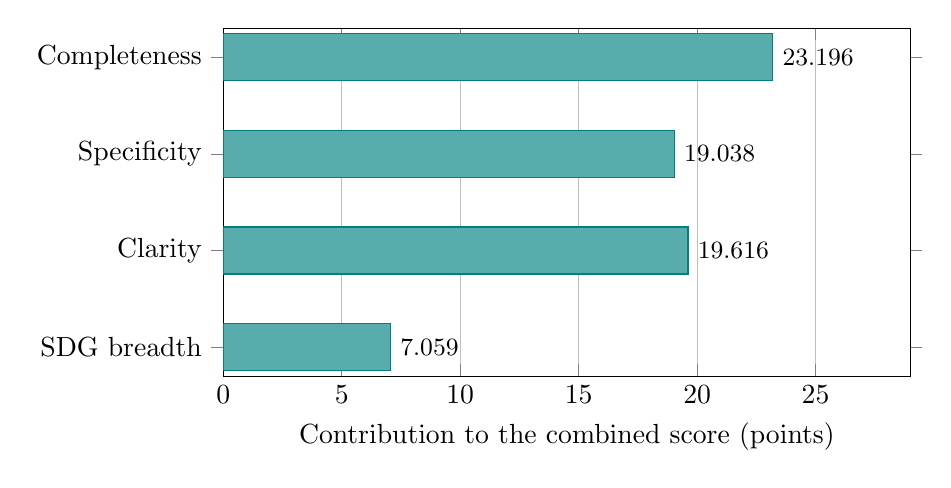
\begin{tikzpicture}
\begin{axis}[width=0.85\linewidth,height=6cm,xbar,bar width=17pt,
  xlabel={Contribution to the combined score (points)},xmin=0,xmax=29,
  symbolic y coords={SDG breadth,Clarity,Specificity,Completeness},ytick=data,xmajorgrids=true,
  nodes near coords,nodes near coords style={font=\small,/pgf/number format/fixed,/pgf/number format/precision=3}]
\addplot[fill=teal!65,draw=teal] coordinates {(7.059,SDG breadth)(19.616,Clarity)(19.038,Specificity)(23.196,Completeness)};
\end{axis}
\end{tikzpicture}
\caption{How the Triveni Turbine score is calculated. Each bar is the component percentage multiplied by the fixed weight. Completeness adds 23.196 points, Specificity 19.038, Clarity 19.616, and SDG breadth 7.059. The total is 68.909, rounded to 68.91. The bars show each component's contribution to the combined score.}
\label{fig:company_contributions}
\end{figure}
